\section{Model}
\label{sec:model}

\begin{figure}[!t]
  \centering
  
\includegraphics[width=0.92\linewidth]{figures/architecture.pdf}
  \caption{AmphionASR architecture.
    A 16\,kHz waveform is encoded by the \textbf{AuT encoder} into the
    language backbone's embedding space; the text branch tokenises the
    instruction and optional hotword lines.
    The audio placeholder is replaced by the audio embedding
    span before next-token prediction.
  A parallel \textbf{RAG} branch retrieves a top-$K$ hotword
    subset from a deployment-scale database and injects it into the
    prompt line; the RAG adapters and the LLM are updated at
    fine-tuning time, and the AuT encoder is also updated in Stage~1
    only and frozen thereafter.}
  \label{fig:architecture}
\end{figure}

\begin{figure}[!t]
  \centering
  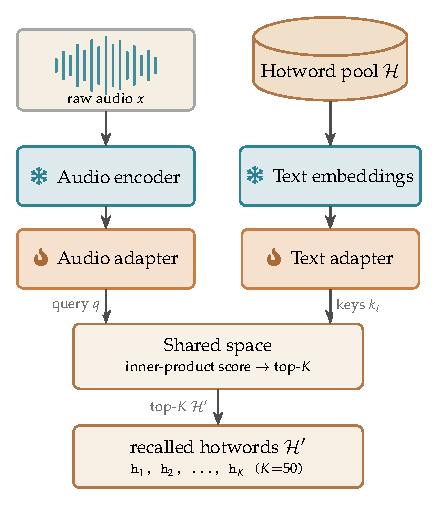
\includegraphics[width=0.58\linewidth]{figures/retrieve.pdf}
  \caption{Retrieval-based contextual biasing paradigm (AmphionASR).
    Frozen acoustic and text features pass through two small trainable
    adapters into a shared embedding space; inner-product scores rank
    the global hotword pool $\mathcal{H}$ and the top-$K$ subset
    $\mathcal{H}'$ is written into the hotword prompt line
    before a \emph{single} ASR forward pass.}
  \label{fig:retrieve}
\end{figure}

\subsection{Overview}

AmphionASR adopts the Qwen3-ASR architecture
\cite{qwen2025qwen3asr}: an AuT audio encoder feeds frame
embeddings directly into the Qwen3-ASR-1.7B language backbone.
At inference time a RAG module retrieves a top-$K$ hotword subset
from a deployment-scale database and writes it into the prompt before
decoding, as shown in Figure~\ref{fig:architecture}.

Component-level parameter counts are summarised in
Table~\ref{tab:params}. AmphionASR totals
$2.0$\,B parameters ($1.7$\,B in the language
backbone plus $0.3$\,B in the audio encoder).

\begin{table}[t]
  \caption{Per-component parameter counts.}
  \label{tab:params}
  \centering
  \small
  \begin{tabular}{lrl}
    \toprule
    Component & Parameters & Detail \\
    \midrule
    AuT encoder               & $300$\,M     & Qwen3-ASR 24-layer AuT encoder \\
    Language model             & $1.7$\,B & Qwen3-ASR-1.7B text backbone (28 layers, 2048-d) \\
    RAG adapter                & $2.6$\,M & two MLP adapters \\
    \midrule
    Total                      & $2.0$\,B & AuT encoder + language backbone + RAG adapter \\
    \bottomrule
  \end{tabular}
\end{table}

\subsection{AuT Audio Encoder}
\label{subsec:audio-encoder}

The acoustic front-end is the Qwen3-ASR \textbf{AuT encoder}
\cite{qwen2025qwen3asr}: a single stack that maps 16\,kHz mono audio
through a log-mel front-end (128 mel bins, 10\,ms hop), a
convolutional sub-sampler and a 24-layer Whisper-style pre-LN
Transformer into 2048-dimensional frame embeddings at
$12.5$\,Hz.
A chunked-inference window of 800 frames extends the effective input
duration beyond the standard 30\,s ceiling.
The AuT encoder is updated only in Stage~1 of fine-tuning and frozen
thereafter; Stages~2--3 update only the language backbone.

\subsection{Language Model}
\label{subsec:llm}

The decoder is the Qwen3-ASR-1.7B text backbone \cite{qwen2025qwen3asr},
a 28-layer decoder-only Transformer with 2048-dimensional hidden
states and a 64\,K native context length. The language backbone is
updated during fine-tuning as described in
Section~\ref{sec:training}.

\subsection{Hotword RAG}
\label{subsec:hotword-rag}

LLM-based ASR can exploit in-prompt contextual biasing---injecting a
hotword list into the prompt---to lift recognition of rare or
domain-specific entities. At deployment scale this naively fails:
writing the whole hotword pool into the prompt overflows the context
window---at which point decoding degrades sharply---and, short of
that, floods the prompt with distractors that the decoder wrongly
inserts, lowering rather than improving accuracy. The remedy is to
first retrieve a small, utterance-relevant hotword subset.

CLAP~\cite{elizalde2023clap} establishes the contrastive
language-audio recipe: two encoders align audio and text in a shared
embedding space, and an audio--text inner product scores relevance.
Applied to hotword retrieval, however, pooling the whole utterance
into a single audio token yields one global query, which loses
temporal locality and performs poorly on long audio or on utterances
that contain several hotwords appearing in short spans.

Following GLCLAP~\cite{kong2025glclap}, AmphionASR retrieves hotwords
with a fine-grained local scoring module (\Cref{fig:retrieve}) that
reuses the frozen AuT audio encoder and the frozen LLM text embedding
table. Two small trainable MLP adapters map these frozen
representations into a shared $512$-dimensional space; the audio side
is kept at the frame level (no utterance-level pooling), and each
candidate hotword is scored against every frame,
\begin{equation}
\begin{aligned}
  \mathbf{a}_t &= g_{\mathrm{audio}}\!\big(\mathrm{AuT}(x)_t\big), \quad
  \mathbf{k}_h = g_{\mathrm{text}}\!\big(\mathbf{E}_{\mathrm{tok}}(h)\big),\\
  s_h &= \max_{t}\, \mathbf{a}_t^{\top}\mathbf{k}_h, \quad
  \mathcal{H}' = \mathrm{TopK}_{h\in\mathcal{H}}\, s_h.
\end{aligned}
  \label{eq:rag-score}
\end{equation}
where $g_{\mathrm{audio}}$ and $g_{\mathrm{text}}$ are the two
adapters, $\mathbf{a}_t$ is the per-frame audio embedding,
$\mathbf{E}_{\mathrm{tok}}$ is the LLM token embedding table, and
$\mathcal{H}'$ is the retrieved top-$K$ subset. The max-over-time
reduction $s_h$ lets an entity that appears only in a short span still
score strongly, and the top-$K$ over hotwords keeps the prompt compact.
The selected hotwords are written into the prompt line before a
\emph{single} ASR forward pass, with no second
transcription~\cite{an2025funasr}.

\subsection{Chat Template}
\label{subsec:prompt}

Each task is exposed to the LLM as a short instruction line followed
by the audio placeholder (Table~\ref{tab:tasks}). AmphionASR
distinguishes plain ASR, hotword ASR, target-speaker ASR, and
whispered ASR purely through this instruction and the presence of
optional prompt fields---the model itself is unchanged. Whispered
speech simply swaps the instruction to ``\textit{Transcribe the
following whispered audio.}''; the other two non-trivial tasks add
prompt fields as below.

\begin{table}[t]
  \caption{Task prompt templates used by AmphionASR. \texttt{\{speech\}}
    denotes the audio placeholder that the merge step fills with the
    encoder-output embedding span; \texttt{\{enroll\}} denotes the
    enrollment utterance.}
  \label{tab:tasks}
  \centering
  \small
  \setlength{\tabcolsep}{4pt}
  \begin{tabular}{lp{9.6cm}}
    \toprule
    Task & Prompt template \\
    \midrule
    Plain ASR        & \texttt{Transcribe the following audio.\{speech\}} \\
    Hotword ASR      & \texttt{Transcribe the following audio.[Hotwords:...].\{speech\}} \\
    TS-ASR           & \texttt{Given the speaker's voice:\{enroll\} Transcribe what this speaker says in the following audio.\{speech\}} \\
    Whisper ASR      & \texttt{Transcribe the following whispered audio.\{speech\}} \\
    \bottomrule
  \end{tabular}
\end{table}

\paragraph{Target-speaker conditioning.}
TS-ASR prepends an enrollment audio block before the main audio and
switches the instruction to ``\textit{Transcribe what this speaker
says in the following audio.}''. Both audio segments share the same
AuT encoder path and reach the LLM as two ordered audio-embedding
spans (enrollment first, mixed audio second).

\paragraph{Hotword conditioning.}
Hotword conditioning is applied purely through the prompt: the
retrieved hotwords are injected as a single comma-separated hotword
line after the instruction, biasing the decoder toward the listed
entities without any architectural change. The list carries no
dedicated delimiter, so the LLM must learn the \verb|Hotwords:|
literal as part of the prompt grammar.

\FloatBarrier
